\documentclass[../report.tex]{subfiles}
\begin{document}

\section{Design of the Sokoban Puzzle Path Planner} \label{sec:solver}
In this section, an algorithm for solving a sokoban puzzle is outlined. To solve a sokoban puzzle a graph search algorithm is used, the search creates a directed graph of states, thus the game must be represented as a search graph.

The Sokoban map is a two dimensional area that contains walls, jewels, goals, a player and free space. The walls indicate the constraint of the map. The jewels can be pushed around by the player. The goals are the desired placement of the jewels. The player can only perform the actions: up, down, right and left.

How the Sokoban puzzle is represented as a search graph and the algorithm to solve the sokoban puzzle will be outlined in \ref{subsec:sokoban_alg}. Lastly, the developed Sokoban puzzle path planner will be evaluated in \ref{subsec:sokoban_eval}.

\subsection{The Algorithm to Solve a Sokoban Puzzle} \label{subsec:sokoban_alg}
The object of the sokoban puzzle is to reach a specified goal state, such that all the jewels are placed on the goals. The formulations are as follows:
\begin{itemize}
    \item \textbf{States:} A state description specifies the location of the player and the jewels.
    \item \textbf{Initial state:} Any state can be designated as the initial state.
    \item \textbf{Actions:} The simplest formulation defines the actions as movements of the free space: left, right, up or down.
    \item \textbf{Transition model:} Given a state and action, this returns the resulting state. For example, in Figure \ref{subfig:inital_state} if the action left is applied, the resulting state would have the M moved one to the left.
    \item \textbf{Goal test:} This checks if the state matches the goal state shown in Figure \ref{subfig:goal_state}.
    \item \textbf{Path cost:} Each step cost one, so the path cost is the number of steps in the path.
\end{itemize}

\begin{figure}[H]
    \centering
    \begin{subfigure}{0.49\textwidth}
        \centering
        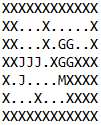
\includegraphics[width=0.3\textwidth]{figures/solver_design/map5.png}
        \caption{Initial state of the sokoban puzzle.}
        \label{subfig:inital_state}
    \end{subfigure}
    \begin{subfigure}{0.49\textwidth}
        \centering
        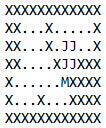
\includegraphics[width=0.3\textwidth]{figures/solver_design/goal_state.png}
        \caption{Goal state of the sokoban puzzle.}
        \label{subfig:goal_state}
    \end{subfigure}
    \caption{Illustration of inital state and goal state of a sokoban puzzle. The "X" represents a wall, "J" represents a jewel, "G" represents a goal, "." represents free space and "M" represents the player.}
    \label{fig:inital_goal_state}
\end{figure}

When working with search graphs the amount of memory in each node must be considered, because the number of nodes can become very high when working with complex problems. Thus, it is desired to only store the necessary data in each of the reached states at each node. 

It was chosen to store the previous state, the jewels positions, the player position and the action of the current state as stated above. Furthermore, it was chosen to use a breadth-first search algorithm to solve the sokoban puzzle. The information is stored in an object, where each object points at the previous object. Thus, by backtracking through the objects, from the goal state, a solution sequence of actions to the sokoban puzzle is found. This sokoban solver is referred to as solver 1 in Section \ref{subsec:sokoban_eval}.

However, solver 1 was not deemed fast enough thus a second algorithm was implemented and tested. The second algorithm has inspiration from \cite{sokoban_solver}. Each node in the second algorithm stores the player position, wall, jewels and free space as a string. Furthermore, the sequence from the initial state to the current state is stored for each node, thus no backtracking is needed. Moreover, some optimized functions in python are also used. This sokoban solver is referred to as solver 2 in Section \ref{subsec:sokoban_eval}.

\subsection{Performance Evaluation of the Implemented Solver} \label{subsec:sokoban_eval}
To evaluate the implemented sokoban puzzle solvers five different maps are used. The maps used are illustrated in \autoref{fig:maps_for_eval}. The "X" character represents a wall, the "G" character represents a goal, the "J" character represents a jewel and the "M" character represents the player.

\begin{figure}[H]
    \centering
    \begin{subfigure}[b]{0.19\textwidth}
        \centering
        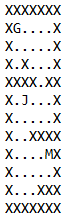
\includegraphics[width=0.5\textwidth]{figures/solver_design/map1.png}
        \captionsetup{width=0.9\textwidth}
        \caption{Map 1.}
        \label{subfig:map1}
    \end{subfigure}
    \begin{subfigure}[b]{0.19\textwidth}
        \centering
        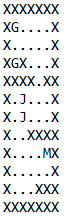
\includegraphics[width=0.5\textwidth]{figures/solver_design/map2.png}
        \captionsetup{width=0.9\textwidth}
        \caption{Map 2.}
        \label{subfig:map2}
    \end{subfigure}
    \begin{subfigure}[b]{0.19\textwidth}
        \centering
        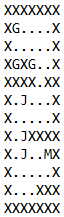
\includegraphics[width=0.5\textwidth]{figures/solver_design/map3.png}
        \captionsetup{width=0.9\textwidth}
        \caption{Map 3.}
        \label{subfig:map3}
    \end{subfigure}
    \begin{subfigure}[b]{0.19\textwidth}
        \centering
        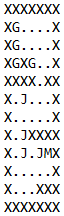
\includegraphics[width=0.5\textwidth]{figures/solver_design/map4.png}
        \captionsetup{width=0.9\textwidth}
        \caption{Map 4.}
        \label{subfig:map4}
    \end{subfigure}
    \begin{subfigure}[b]{0.19\textwidth}
        \centering
        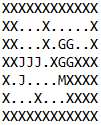
\includegraphics[width=0.75\textwidth]{figures/solver_design/map5.png}
        \captionsetup{width=0.9\textwidth}
        \caption{Map 5.}
        \label{subfig:map5}
    \end{subfigure}
    \caption{Maps used for performance evaluation of the implemented solvers.}
    \label{fig:maps_for_eval}
\end{figure}

In \autoref{fig:maps_for_eval}, the five different maps has different number of jewels, thus the complexity of the maps rises from \autoref{subfig:map1} to \autoref{subfig:map5}. Each solver was stopped if it exceeded $15$ minutes, as this was deemed the maximum acceptable solving time.

\begin{table}[H]
\centering
\resizebox{\textwidth}{!}{%
\begin{tabular}{l|ccc|ccc}
\toprule
\multirow{2}{*}{Map} & \multicolumn{3}{c|}{Solver 1} & \multicolumn{3}{c}{Solver 2} \\
& Time {[}s{]} & Memory usage {[}MB{]} & Solved? & Time {[}s{]} & Memory usage {[}MB{]} & Solved? \\ \hline
Map 1 & 0.491 & 29.282 & True & 0.0101 & 11.788 & True \\
Map 2 & 94.665 & 104.821 & True & 0.343 & 14.852 & True \\
Map 3 & 900.343 & 327.049 & False & 4.700 & 28.484 & True \\
Map 4 & 900.499 & 479.531 & False & 42.808 & 110.637 & True \\
Map 5 & 900.451 & 496.239 & False & 18.781 & 99.533 & True \\ \bottomrule
\end{tabular}
}
\caption{Results of performance evaluation of the implemented solvers on the maps shown in \autoref{fig:maps_for_eval}.}
\label{tab:solver_results}
\end{table}

From \autoref{tab:solver_results}, solver 2 is faster than solver 1 and it uses less memory. For example, in map 1 solver 2 has a $97.9\ \%$ decrease in time compared to solver 1. Furthermore, solver 2 has a $59.7\ \%$ decrease in memory usage compared to solver 1 on map 1. On map 2 the decrease in time, from solver 2 to solver 1, is $99.6\ \%$ and the decrease in memory is $85.8\ \%$. However, on maps 3, 4 and 5 solver 1 could not find a solution in under $15$ minutes. Based on the results solver 2 is used.

\end{document}